\documentclass[10pt,pdf,hyperref={unicode}]{beamer}

\mode<presentation>
{
\usetheme{boxes}
\beamertemplatenavigationsymbolsempty

\setbeamertemplate{footline}[page number]
\setbeamersize{text margin left=1em, text margin right=1em}
}

\usepackage[T2A]{fontenc}
\usepackage[utf8]{inputenc}
\usepackage[english, russian]{babel}
\usepackage{bm}
\usepackage{multirow}
\usepackage{ragged2e}
\usepackage{indentfirst}
\usepackage{multicol}
\usepackage{subfig}
\usepackage{amsmath,amssymb}
\usepackage{enumerate}
\usepackage{mathtools}
\usepackage{comment}
\usepackage{multicol}
\usepackage{color}
\usepackage{graphicx}
\usepackage{booktabs}
\definecolor{python-green}{RGB}{55,126,33}

\usepackage[all]{xy}

\usepackage{tikz}
\usetikzlibrary{positioning,arrows}

\usepackage{caption}
\captionsetup{skip=0pt,belowskip=0pt}

\newtheorem{rustheorem}{Теорема}
\newtheorem{ruslemma}{Лемма}
\newtheorem{russtatement}{Утверждение}
\newtheorem{rusdefinition}{Определение}
\newtheorem{rusassumption}{Предположение}
\newtheorem{rusremark}{Замечание}
\newtheorem{ruscorollary}{Следствие}

% colors
\definecolor{darkgreen}{rgb}{0.0, 0.2, 0.13}
\definecolor{darkcyan}{rgb}{0.0, 0.55, 0.55}

\AtBeginEnvironment{figure}{\setcounter{subfigure}{0}}%

%----------------------------------------------------------------------------------------------------------

\title[Ландшафтная мера сложности]{%
О ландшафтной мере сложности для полносвязных сетей ReLU при квадратичной функции потерь}

\author{%
    Андрей Грабовой}

\institute[ИПУ РАН]{%
Институт Проблем Управления РАН им. Трапезникова\\
grabovoy@ipu.ru}

\date{29.05.2026}

%---------------------------------------------------------------------------------------------------------
\begin{document}

\begin{frame}
\titlepage
\end{frame}

%----------------------------------------------------------------------------------------------------------
\begin{frame}{Ландшафтная мера сложности для полносвязных ReLU сетей}
\justifying
Исследуется связь между локальной геометрией функции потерь и классическими мерами емкости в задачах регрессии.

\begin{block}{Задача}
\justifying
Анализ ландшафта функции потерь и его соотношения с равномерной сложностью для скалярной регрессии полносвязных ReLU сетей при квадратичной ошибке.
\end{block}

\begin{block}{Цель}
\justifying
Разработать ландшафтную меру сложности, отражающую локальную вариативность Гессиана вокруг эмпирического среднего, и исследовать ее масштабирование.
\end{block}

\begin{block}{Метод}
\justifying
Определение ландшафтной меры сложности через спектральную дисперсию Гессианов, вывод законов масштабирования по глубине, ширине и ограничениям нормы, теоретическое сравнение с эмпирической сложностью Радемахера; численная верификация.
\end{block}
\end{frame}

%----------------------------------------------------------------------------------------------------------
\begin{frame}{Постановка задачи}
\justifying
Заданы
\begin{enumerate}[1)]
    \item Выборка $D=\{(\mathbf{x}_i,y_i)\}_{i=1}^{m}$, $\mathbf{x}_i\in\mathbb{R}^n$, $y_i\in\mathbb{R}.$
    \item $L$-слойная полносвязная нейронная сеть с функцией активации ReLU,
    \[
        f_{\boldsymbol{\theta}}(\mathbf{x})=\mathbf{W}^{(L)}\sigma\bigl(\cdots\sigma(\mathbf{W}^{(1)}\mathbf{x})\bigr),
        \qquad \boldsymbol{\theta}\in\mathbb{R}^P.
    \]
    \item Ошибка на объектах и риск на первых $k$ объектах выборки:
    \[
        \ell_i(\boldsymbol{\theta})
        = \tfrac{1}{2}\bigl(f_{\boldsymbol{\theta}}(\mathbf{x}_i)-y_i\bigr)^2,
        \qquad
        \mathcal{L}_k(\boldsymbol{\theta})
        = \frac{1}{k}\sum_{i=1}^{k}\ell_i(\boldsymbol{\theta}),
        \quad k=1,\ldots,m .
    \]
\end{enumerate}
Гессиан на объектах выборки:
\[
    \mathbf{H}_i(\boldsymbol{\theta})
    =\nabla^2_{\boldsymbol{\theta}}\ell\bigl(f_{\boldsymbol{\theta}}(\mathbf{x}_i),y_i\bigr).
\]
Ограничения на параметры $f_{\boldsymbol{\theta}}$: $\|\mathbf{W}^{(p)}\|_2\le M_{\mathbf{W}}$, $\|\mathbf{x}_i\|_2\le M_{\mathbf{x}}$.

Рассматриваемая точка локального минимума $\boldsymbol{\theta}^*$.
\end{frame}

%----------------------------------------------------------------------------------------------------------
\begin{frame}{Ландшафтная мера сложности}
\justifying
Рассматривается матрица Гессе для~$k$ объектов выборки:
\[
    \mathbf{H}^{(k)}(\boldsymbol{\theta})
    =\frac{1}{k}\sum_{i=1}^{k}\mathbf{H}_i(\boldsymbol{\theta}),
    \qquad
    \bar{\mathbf{H}}(\boldsymbol{\theta})
    =\frac{1}{m}\sum_{i=1}^{m}\mathbf{H}_i(\boldsymbol{\theta}) .
\]

\begin{rusdefinition}
Ландшафтная мера сложности на выборке $D$ в точке $\boldsymbol{\theta}^*$:
\[
    \mu_f(f\mid D)
    =\frac{1}{m}\sum_{i=1}^{m}
    \left\|
    \mathbf{H}_{i}(\boldsymbol{\theta}^*)
    -\bar{\mathbf{H}}(\boldsymbol{\theta}^*)
    \right\|_2
    =\mathsf{E}_{i\in D}\left\|
    \mathbf{H}_{i}(\boldsymbol{\theta}^*)
    -\bar{\mathbf{H}}(\boldsymbol{\theta}^*)
    \right\|_2 .
\]
\end{rusdefinition}

Мера~$\mu_f$ описывает разброс $\mathbf{H}_i$ относительно $\bar{\mathbf{H}}$ в спектральной норме.
\end{frame}

%----------------------------------------------------------------------------------------------------------
\begin{frame}{Приращение риска при добавлении объекта}
\justifying
\begin{rusassumption}
Для некоторого $\varepsilon_g\ge 0$,
\begin{equation}\label{eq:eps-g}
  \bigl\|\nabla \mathcal{L}_k(\boldsymbol{\theta}^*)\bigr\|_2 \le \varepsilon_g,
  \qquad
  \bigl\|\nabla \mathcal{L}_{k+1}(\boldsymbol{\theta}^*)\bigr\|_2 \le \varepsilon_g .
\end{equation}
\end{rusassumption}

В условиях предположения справедлива оценка на изменение ландшафта:
\[\begin{aligned}
  \bigl|\mathcal{L}_{k+1}(\boldsymbol{\theta})-\mathcal{L}_k(\boldsymbol{\theta})\bigr|
  &\le \frac{1}{k+1}\Bigl|\ell_{k+1}(\boldsymbol{\theta}^*)-\bar{\ell}_k(\boldsymbol{\theta}^*)\Bigr| \\
  &\quad + \frac{\|\boldsymbol{\theta}-\boldsymbol{\theta}^*\|_2^2}{k+1}
    \left\| \mathbf{H}_{k+1}(\boldsymbol{\theta}^*)-\mathbf{H}^{(k)}(\boldsymbol{\theta}^*) \right\|_2 \\
  &\quad + 2\varepsilon_g\|\boldsymbol{\theta}-\boldsymbol{\theta}^*\|_2 .
\end{aligned}\]
\end{frame}

%----------------------------------------------------------------------------------------------------------
\begin{frame}{Гессиан при среднеквадратичной ошибке}
\justifying
Пусть $u_i=f_{\boldsymbol{\theta}}(\mathbf{x}_i)$, $\ell(u,y)=\tfrac12(u-y)^2$. Тогда
\[
    \mathbf{H}_i(\boldsymbol{\theta})
    =\nabla_{\boldsymbol{\theta}}u_i\,\nabla_{\boldsymbol{\theta}}u_i^{\top}
    +(u_i-y_i)\,\nabla_{\boldsymbol{\theta}}^2 u_i .
\]
При среднеквадратичной ошибке $\partial^2\ell/\partial u^2=1$.

Из разложения следует
\[
    \|\mathbf{H}_i(\boldsymbol{\theta})\|_2
    \le \|\nabla_{\boldsymbol{\theta}}u_i\|_2^2
    +|u_i-y_i|\,\|\nabla_{\boldsymbol{\theta}}^2 u_i\|_2 .
\]

\begin{ruslemma}
Для полносвязной сети с функцией активации ReLU при $\|\mathbf{W}^{(p)}\|_2\le M_{\mathbf{W}}$ и $\|\mathbf{x}_i\|_2\le M_{\mathbf{x}}$ справедлива оценка матрицы Гессе:
\[
    \|\mathbf{H}_i(\boldsymbol{\theta})\|_2
    \le M_{\mathbf{H}}
    := L M_{\mathbf{x}}^2 M_{\mathbf{W}}^{2L}
    +\sum_{s=1}^{L} M_{\mathbf{W}}^{2s}.
\]
При~$|w_{ij}^{(p)}|\le M$ с размерностью слоев~$h\times h$:
$\|\mathbf{H}_i(\boldsymbol{\theta})\|_2=O\!\bigl(L(hM)^{2L}\bigr)$.
\end{ruslemma}
\end{frame}

%----------------------------------------------------------------------------------------------------------
\begin{frame}{Теорема о приращении риска}
\justifying
\begin{rustheorem}
Пусть параметр $\boldsymbol{\theta}$ удовлетворяет условию $\|\boldsymbol{\theta}-\boldsymbol{\theta}^*\|_2\le R$.
Пусть ошибка на всех объектах удовлетворяет условию $\bigl|\ell(f_{\boldsymbol{\theta}^*}(\mathbf{x}_i),\mathbf{y}_i)\bigr|\le M_{\ell}$, также условие Леммы и предположения выполняются для некоторого $\varepsilon_g\ge 0$.
Тогда справедлива оценка
\[
  \bigl|\mathcal{L}_{k+1}(\boldsymbol{\theta}) - \mathcal{L}_k(\boldsymbol{\theta})\bigr|
  \le \frac{2}{k+1}\bigl( M_{\ell} + M_{\mathbf{H}} R^2 \bigr) + 2\,\varepsilon_g\, R .
\]
В худшем случае оценка принимает вид
$\bigl|\mathcal{L}_{k+1}(\boldsymbol{\theta}) - \mathcal{L}_k(\boldsymbol{\theta})\bigr|\;=\; O\!\left(\frac{L(hM)^{2L} R^2}{k}\right).$
При выполнении дополнительного условия для каждого объекта выборки
$\bigl|f_{\boldsymbol{\theta}^*}(\mathbf{x}_i)-y_i\bigr|\le \varepsilon_y.$
Справедлива оценка
\[
  \bigl|\mathcal{L}_{k+1}(\boldsymbol{\theta}) - \mathcal{L}_k(\boldsymbol{\theta})\bigr|
  \le
  \frac{\varepsilon_y^2 + 2R^2\bigl(L M_{\mathbf{x}}^2 M_{\mathbf{W}}^{2L-2} + \varepsilon_y M_{\nabla^2 f}\bigr)}{k+1}
  + 2\,\varepsilon_g\,R .
\]
\end{rustheorem}
\end{frame}

%----------------------------------------------------------------------------------------------------------
\begin{frame}{Масштабирование ландшафтной меры сложности}
\justifying
\begin{ruscorollary}
При условиях леммы, $|w_{ij}^{(p)}|\le M$ на слоях размера~$h\times h$ и фиксированной норме входов:
\[
\mu_f(f\mid D)=O\!\bigl(L(hM)^{2L}\bigr).
\]
\end{ruscorollary}

\begin{ruscorollary}[Линейная модель]
Пусть $f_{\boldsymbol{\theta}}(\mathbf{x})=\mathbf{w}^{\top}\mathbf{x}$, $\boldsymbol{\theta}=\mathbf{w}\in\mathbb{R}^n$. Тогда
$\mu_f(f\mid D)\le 2\max_{1\le i\le m}\|\mathbf{x}_i\|_2^2.$
~\\
Если, также, $\|\mathbf{x}_i\|_2^2=\Theta(n)$ при $n\to\infty$, то $\mu_f(f\mid D)=O(n)$.
\end{ruscorollary}

\begin{ruscorollary}[Однослойный персептрон]
Для полносвязной сети с функцией активации ReLU с одним скрытым слоем $L=2$ ширины $h$ получаем
$\mu_f(f\mid D)=O\!\bigl((hM)^4\bigr)$.
При $|f_{\boldsymbol{\theta}^*}(\mathbf{x}_i)-y_i|\le\varepsilon_y$ и условиях теоремы о приращении риска:
\[
\mu_f(f\mid D)
\le 2hM^2\max_{1\le i\le m}\bigl(\|\mathbf{x}_i\|_1^2+\|\mathbf{x}_i\|_2^2\bigr)
+2\varepsilon_y M_{\nabla^2 f}.
\]
Если $\|\mathbf{x}_i\|_2^2=\Theta(n)$ и $\|\mathbf{x}_i\|_1=\Theta(n)$, то
$\mu_f(f\mid D)=O\!\bigl(hM^2n^2+\varepsilon_y M_{\nabla^2 f}\bigr)$.
\end{ruscorollary}
\end{frame}

%----------------------------------------------------------------------------------------------------------
\begin{frame}{Сравнение порядков роста}
\justifying
$\mu_f$ отвечает за локальный разброс Гессианов в $\boldsymbol{\theta}^*$.
~\\
$\hat{\mathfrak{R}}_m$ --- за емкость класса $\mathcal{F}$ на $D$.

\begin{table}
\centering
\setlength{\tabcolsep}{6pt}
\begin{tabular}{@{}lcc@{}}
\toprule
 & Линейная модель & Однослойный персептрон \\
\midrule
$\mu_f(f\mid D)$ & $O(n)$ & $O((hM)^4)$ или $O(hM^2n^2)$ \\
\addlinespace[0.2em]
$\hat{\mathfrak{R}}_m(\mathcal{F})$ &
$O(W\sqrt{n/m})$ &
$O(\mathrm{poly}(h)/\sqrt{m})$ \\
\bottomrule
\end{tabular}
\end{table}

Для линейной модели $\mu_f$ линейна по $n$, а $\hat{\mathfrak{R}}_m$ --- порядка $\sqrt{n}$ при фиксированном~$m$.

Для однослойного перцептрона в $\hat{\mathfrak{R}}_m$ остается множитель $m^{-1/2}$, рост по $h$ --- полиномиальный и обычно мягче, чем наихудший порядок $\mu_f$ по $h$.
\end{frame}

%----------------------------------------------------------------------------------------------------------
\begin{frame}{Линейная модель, размерность $n$}
\justifying
Размер выборки $m=256$, число параметров $n\in[8,128]$, 16 повторов.

\begin{figure}
\centering
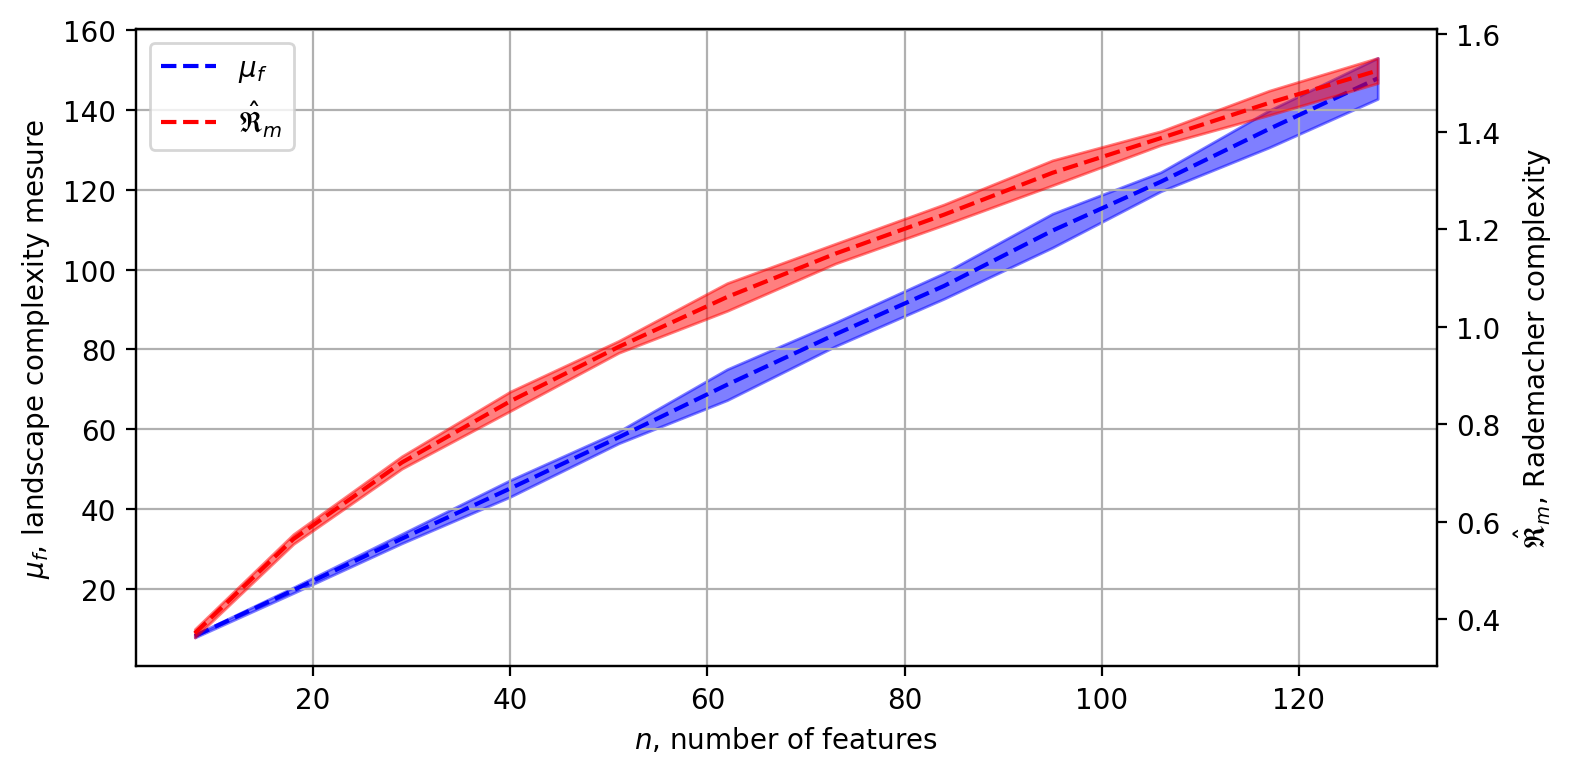
\includegraphics[width=0.78\textwidth]{../figures/exp01_linear_sweep_n.png}
\end{figure}

Две шкалы по $n$ при $m=256$: $\mu_f$ растет примерно линейно, $\hat{\mathfrak{R}}_m$~--- как $\sqrt{n}$.~\\
На слайде~--- контраст роста двух мер при одной линейной модели.
\end{frame}

%----------------------------------------------------------------------------------------------------------
\begin{frame}{Линейная модель, размер выборки $m$}
\justifying

Число признаков~$n=64$, размер выборки $m\in[16,1024]$, 16 повторов.

\begin{columns}[T,onlytextwidth]
\begin{column}{0.49\textwidth}
\centering
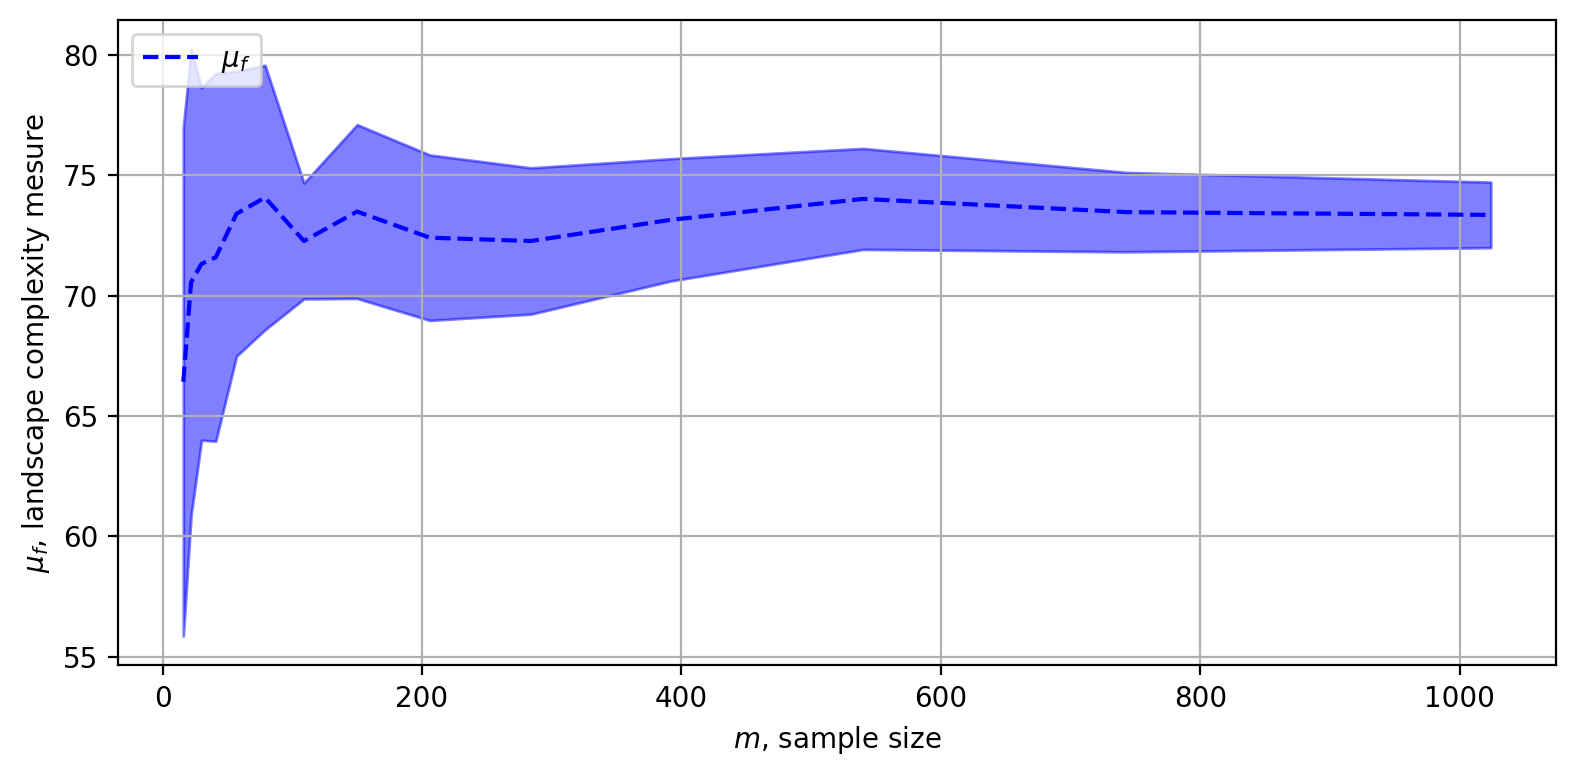
\includegraphics[width=\linewidth]{../figures/exp02_linear_sweep_m_mu.png}
\end{column}
\begin{column}{0.49\textwidth}
\centering
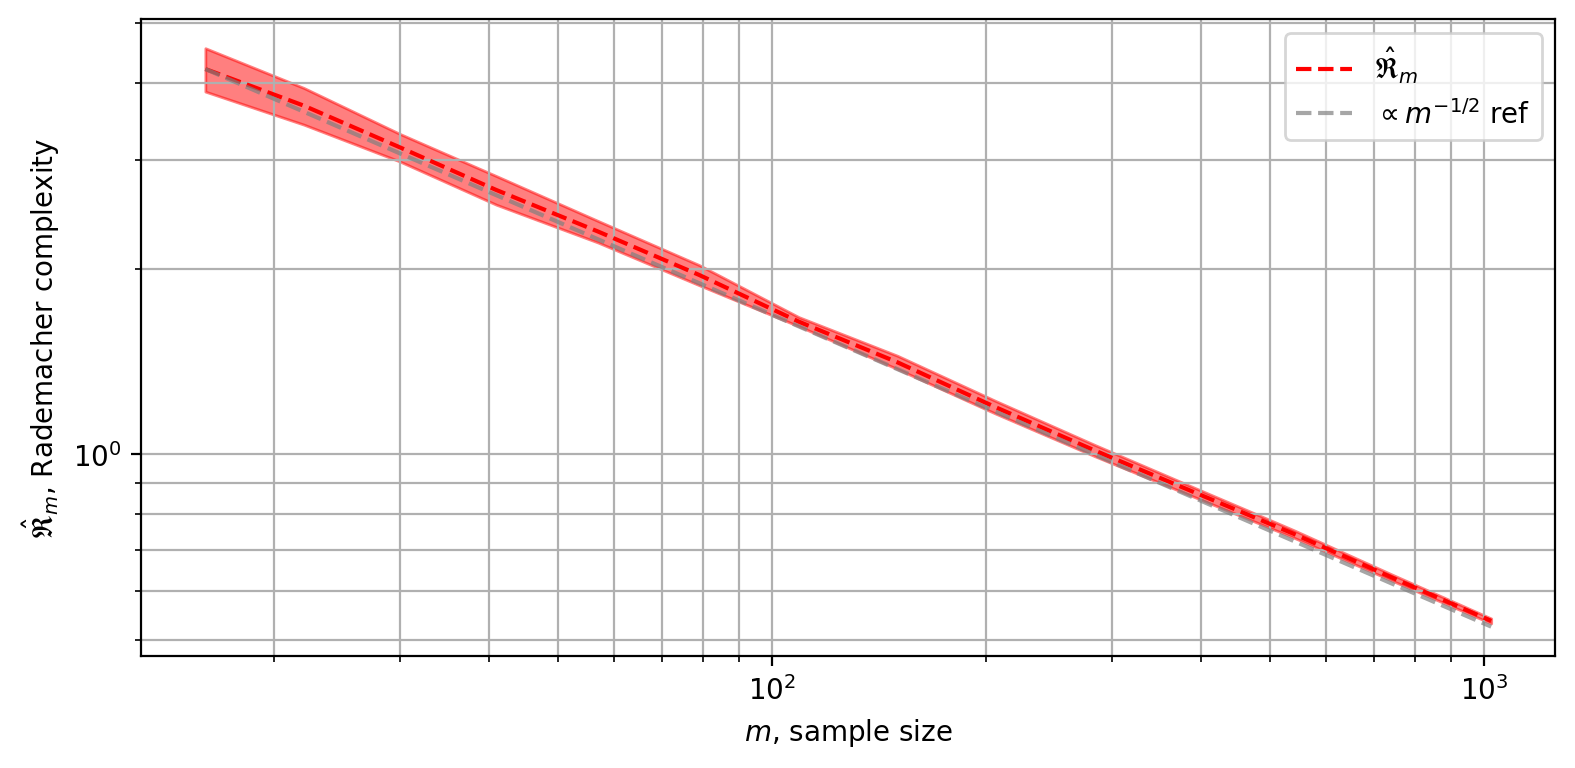
\includegraphics[width=\linewidth]{../figures/exp02_linear_sweep_m_rademacher.png}
\end{column}
\end{columns}

При росте $m$ и фиксированном $n=64$: $\mu_f$ почти не меняется, так как ограничена $\max_i\|\mathbf{x}_i\|_2^2$, а $\hat{\mathfrak{R}}_m$ на log--log убывает как $m^{-1/2}$.~\\
Две меры по-разному реагируют на размер выборки.
\end{frame}

%----------------------------------------------------------------------------------------------------------
\begin{frame}{Однослойный персептрон}
\justifying
\begin{enumerate}
    \item $n=h$, $m=512$, $|w_{ij}|\le M=1$, оценка в $\boldsymbol{\theta}^\star$.
    \item $\mu_f$ --- батчевые поэкземплярные Гессианы, $\hat{\mathfrak{R}}_m$ --- PGD на шаре по весам.
    \item На графике эталоны $\propto(hM)^4$ и $\propto h^3$.
\end{enumerate}

\begin{figure}
\centering
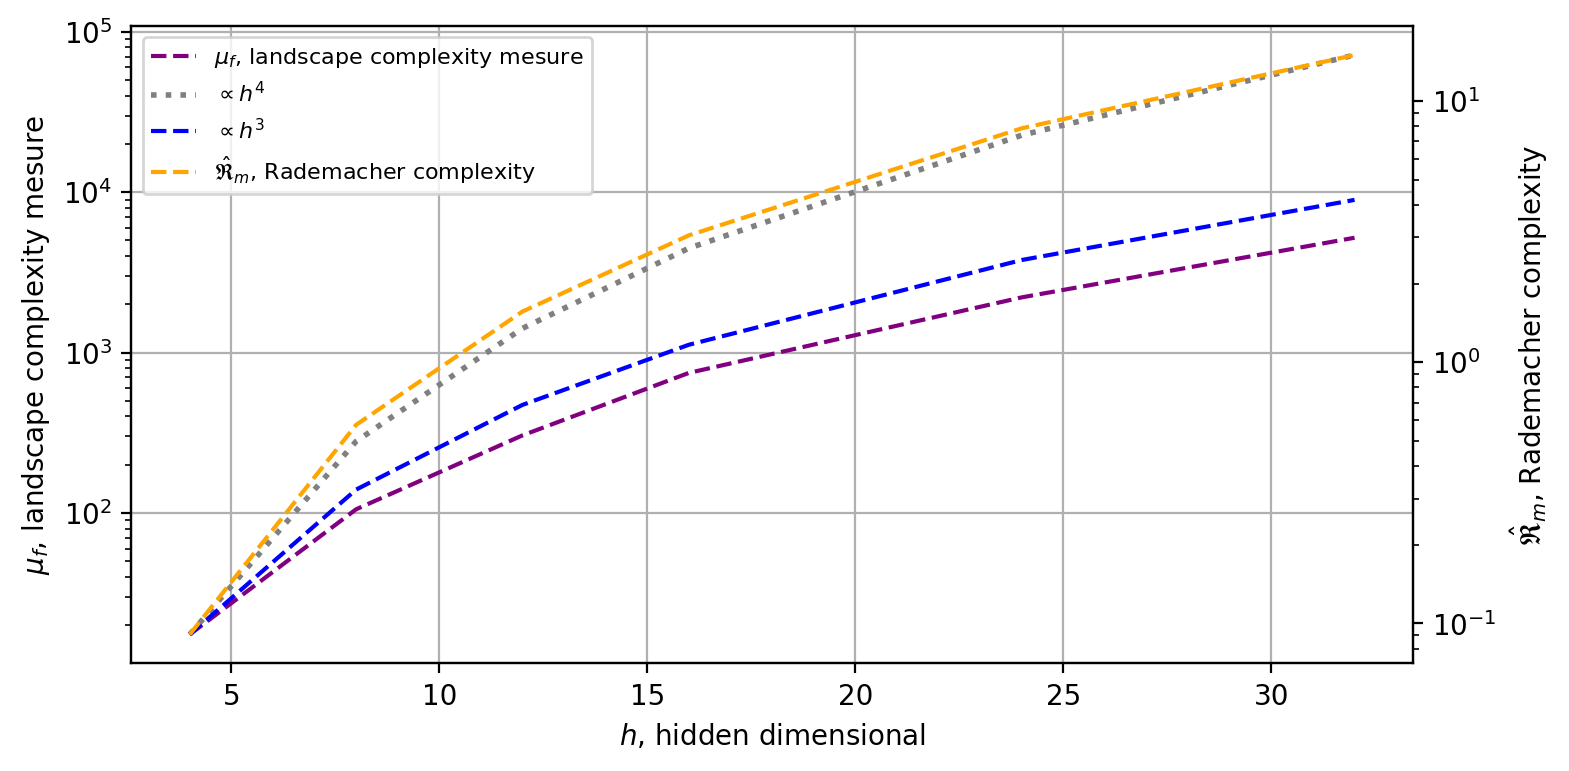
\includegraphics[width=0.78\textwidth]{../figures/exp03_twolayer_sweep_h.png}
\end{figure}

По $h$ при $n=h$: эмпирическая $\mu_f$ ближе к кривой $h^3$, чем к наихудшему случаю $(hM)^4$.~\\
График зависимости~$\hat{\mathfrak{R}}_m$ от $h$ ниже чем $\mu_f$.
\end{frame}

%----------------------------------------------------------------------------------------------------------
\begin{frame}{Заключение}
\justifying
\begin{enumerate}
    \item Предложена ландшафтная мера сложности $\mu_f$~--- спектральная дисперсия поэкземплярных Гессианов для полносвязной сети с функцией активации ReLU при среднеквадратичной ошибке.
    \item Получены законы масштабирования $\mu_f$ по глубине $L$, ширине $h$ и нормам весов.
    \item Показано, что $\mu_f$ и $\hat{\mathfrak{R}}_m$ дополняют, а не дублируют друг друга.
    \item Численные эксперименты согласуются с теорией для линейной модели и однослойного перцептрона.
\end{enumerate}
\end{frame}
%----------------------------------------------------------------------------------------------------------
\begin{frame}{Планы на будущее}
\justifying
\begin{enumerate}
    \item Разработка законов масштабирования больших языковых моделей на основе ландшафтной меры сложности параметрических моделей.
    \item Разработка теории сложности инструментов больших языковых моделей используя текстовые описания инструментов как априорную информацию.
\end{enumerate}
\end{frame}
%----------------------------------------------------------------------------------------------------------
\end{document}